\documentclass{article} % say
\usepackage{tikz}
\begin{document}
\tikzset{help lines/.style=very thin}
\tikzset{Karl's grid/.style={help lines,color=blue!50}}
We are working on
\begin{tikzpicture}
\draw (-1.5,0) -- (1.5,0);
\draw (0,-1.5) -- (0,1.5);
\end{tikzpicture}.

\tikz \draw (-1.5,0) -- (1.5,0) -- (0,-1.5) -- (0,1.5);

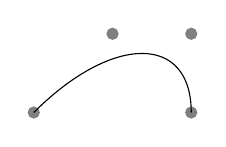
\begin{tikzpicture}
\filldraw [gray] (0,0) circle [radius=2pt]
(1,1) circle [radius=2pt]
(2,1) circle [radius=2pt]
(2,0) circle [radius=2pt];
\draw (0,0) .. controls (1,1) and (2,1) .. (2,0);
\end{tikzpicture}

\begin{tikzpicture}
\filldraw [gray] (-1,0.555) circle [radius=2pt]
(-0.555,1) circle [radius=2pt]
(0.555,1) circle [radius=2pt]
(1,0.555) circle [radius=2pt];
\draw (-1.5,0) -- (1.5,0);
\draw (0,-1.5) -- (0,1.5);
\draw (-1,0) .. controls (-1,0.555) and (-0.555,1) .. (0,1)
.. controls (0.555,1) and (1,0.555) .. (1,0);
\end{tikzpicture}
\tikz \draw (0,0) circle [radius=50pt];
\tikz \draw (0,0) ellipse [x radius=20pt, y radius=10pt];
\tikz \draw[rotate=30] (0,0) ellipse [x radius=10pt, y radius=6pt];

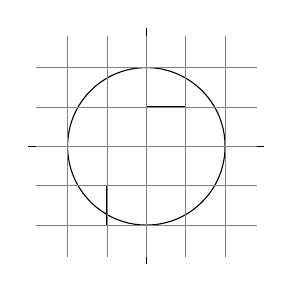
\begin{tikzpicture}
\draw (-1.5,0) -- (1.5,0);
\draw (0,-1.5) -- (0,1.5);
\draw (0,0) circle [radius=1cm];
\draw (0,0) rectangle (0.5,0.5);
\draw (-0.5,-0.5) rectangle (-1,-1);
\draw[step=.5cm,gray,very thin] (-1.4,-1.4) grid (1.4,1.4);
\end{tikzpicture}

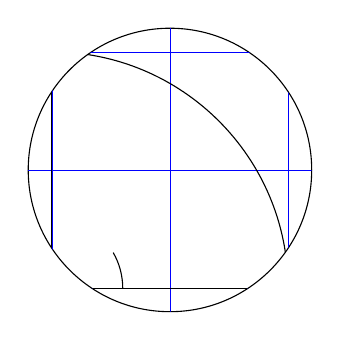
\begin{tikzpicture}[scale=3]
%\clip (-0.1,-0.2) rectangle (1.1,0.75);
\clip[draw] (0.5,0.5) circle (.6cm);
\draw[step=.5cm,blue,very thin] (-1.4,-1.4) grid (1.4,1.4);
\draw (-1.5,0) -- (1.5,0);
\draw (0,-1.5) -- (0,1.5);
\draw (0,0) circle [radius=1cm];
\draw (3mm,0mm) arc [start angle=0, end angle=30, radius=3mm];
\end{tikzpicture}

\tikz \draw (0,0) rectangle (1,1) (0,0) parabola (1,1);
\tikz \draw[x=1pt,y=1pt] (0,0) parabola bend (2,16) (6,12);
A sine \tikz \draw[x=1ex,y=1ex,scale=3] (0,0) sin (1.57,1); curve.
\end{document}